\documentclass[11pt,a4paper]{article}
\usepackage[T2A]{fontenc}
\usepackage[utf8]{inputenc}
\usepackage[english,russian]{babel}
\sloppy
\setlength{\emergencystretch}{2em}
\usepackage[margin=2.1cm]{geometry}
\usepackage{xcolor}
\usepackage{graphicx}
\usepackage{listings}
\usepackage{enumitem}
\usepackage{booktabs}
\usepackage{array}
\newcolumntype{L}[1]{>{\raggedright\arraybackslash}p{#1}}
\usepackage{amsmath}
\usepackage{tikz}
\usetikzlibrary{arrows.meta,positioning,calc,fit,shapes.geometric}
\usepackage{titlesec}
\usepackage{fancyhdr}
\usepackage[hidelinks]{hyperref}
\usepackage{caption}
\captionsetup{font=small,labelfont=bf}
% babel нь \begin{document}-д эдгээрийг дардаг тул AtBeginDocument ашиглана
\AtBeginDocument{%
  \renewcommand{\contentsname}{Гарчиг}%
  \renewcommand{\tablename}{Хүснэгт}%
  \renewcommand{\figurename}{Зураг}%
  \renewcommand{\refname}{Ашигласан материал}%
}

\definecolor{codebg}{RGB}{246,247,249}
\definecolor{accent}{RGB}{31,78,121}

\lstset{
  basicstyle=\ttfamily\footnotesize,
  backgroundcolor=\color{codebg},
  frame=single, rulecolor=\color{gray!40},
  keywordstyle=\color{accent}\bfseries,
  commentstyle=\color{gray}\itshape,
  breaklines=true, columns=fullflexible, keepspaces=true,
  extendedchars=true, inputencoding=utf8,
  literate=
    {А}{{\CYRA}}1
    {Б}{{\CYRB}}1
    {В}{{\CYRV}}1
    {Г}{{\CYRG}}1
    {Д}{{\CYRD}}1
    {Е}{{\CYRE}}1
    {Ё}{{\CYRYO}}1
    {Ж}{{\CYRZH}}1
    {З}{{\CYRZ}}1
    {И}{{\CYRI}}1
    {Й}{{\CYRISHRT}}1
    {К}{{\CYRK}}1
    {Л}{{\CYRL}}1
    {М}{{\CYRM}}1
    {Н}{{\CYRN}}1
    {О}{{\CYRO}}1
    {Ө}{{\CYROTLD}}1
    {П}{{\CYRP}}1
    {Р}{{\CYRR}}1
    {С}{{\CYRS}}1
    {Т}{{\CYRT}}1
    {У}{{\CYRU}}1
    {Ү}{{\CYRY}}1
    {Ф}{{\CYRF}}1
    {Х}{{\CYRH}}1
    {Ц}{{\CYRC}}1
    {Ч}{{\CYRCH}}1
    {Ш}{{\CYRSH}}1
    {Щ}{{\CYRSHCH}}1
    {Ъ}{{\CYRHRDSN}}1
    {Ы}{{\CYRERY}}1
    {Ь}{{\CYRSFTSN}}1
    {Э}{{\CYREREV}}1
    {Ю}{{\CYRYU}}1
    {Я}{{\CYRYA}}1
    {а}{{\cyra}}1
    {б}{{\cyrb}}1
    {в}{{\cyrv}}1
    {г}{{\cyrg}}1
    {д}{{\cyrd}}1
    {е}{{\cyre}}1
    {ё}{{\cyryo}}1
    {ж}{{\cyrzh}}1
    {з}{{\cyrz}}1
    {и}{{\cyri}}1
    {й}{{\cyrishrt}}1
    {к}{{\cyrk}}1
    {л}{{\cyrl}}1
    {м}{{\cyrm}}1
    {н}{{\cyrn}}1
    {о}{{\cyro}}1
    {ө}{{\cyrotld}}1
    {п}{{\cyrp}}1
    {р}{{\cyrr}}1
    {с}{{\cyrs}}1
    {т}{{\cyrt}}1
    {у}{{\cyru}}1
    {ү}{{\cyry}}1
    {ф}{{\cyrf}}1
    {х}{{\cyrh}}1
    {ц}{{\cyrc}}1
    {ч}{{\cyrch}}1
    {ш}{{\cyrsh}}1
    {щ}{{\cyrshch}}1
    {ъ}{{\cyrhrdsn}}1
    {ы}{{\cyrery}}1
    {ь}{{\cyrsftsn}}1
    {э}{{\cyrerev}}1
    {ю}{{\cyryu}}1
    {я}{{\cyrya}}1,
  xleftmargin=0.8em, framexleftmargin=0.8em,
  language=Java, showstringspaces=false
}
\titleformat{\section}{\Large\bfseries\color{accent}}{\thesection}{0.6em}{}
\titleformat{\subsection}{\large\bfseries}{\thesubsection}{0.6em}{}
\pagestyle{fancy}
\fancyhf{}
\fancyfoot[C]{\thepage}
\renewcommand{\headrulewidth}{0.4pt}
\setlength{\headheight}{14pt}
\setlength{\parskip}{3pt}
\fancyhead[L]{\small IV-2-7 --- Fork-Join Sorting Application}
\fancyhead[R]{\small Хэрэглэгчийн заавар}

\begin{document}
\begin{titlepage}
\centering
\vspace*{2.5cm}
{\large F.CSM302 --- Үйлдлийн систем · Бие даалт 1\par}
\vspace{1.4cm}
{\Huge\bfseries\color{accent} Хэрэглэгчийн заавар\par}
\vspace{0.5cm}
{\Large Fork-Join Sorting Application\par}
\vspace{0.3cm}
{\large Хуваарилалтын код: \textbf{IV-2-7} · Сэдэв №7\par}
{\large UI дүрслэл: Recursion tree\par}
\vspace{0.6cm}
{\large Бие даалт 1-ийн 8.1 хэсэг\par}
\vfill
{\large 2026 оны 10-р сар}
\vspace{2cm}
\end{titlepage}

\tableofcontents
\newpage
\section{Хэрэглэгчийн заавар}

\subsection{Программын зорилго}
Энэхүү программ нь Java-гийн \textbf{Fork/Join} параллель API ашиглан массивыг
эрэмбэлэх хоёр алгоритмыг (Mergesort, Quicksort) хэрэгжүүлж, тэдгээрийн
\emph{рекурсив задралыг} модоор харуулна.

Зорилго нь зөвхөн эрэмбэлэх биш --- \emph{параллель ажил хэрхэн хуваагдаж,
аль урсгал ямар хэсгийг гүйцэтгэж, threshold ямар нөлөөтэйг нүдээр харуулах}
явдал юм.

\subsection{Дэмжих орчин}
\begin{center}
\small
\begin{tabular}{lL{10.5cm}}
\toprule
Шаардлага & Утга \\
\midrule
Java & \textbf{JDK 17 буюу түүнээс дээш}. Туршилтыг JDK 21.0.12 дээр хийсэн. \\
Үйлдлийн систем & Linux, macOS, Windows --- Java ажиллах аль ч орчин \\
Гадны сан & \textbf{Байхгүй}. Зөвхөн стандарт JDK. Интернэт шаардлагагүй. \\
Дэлгэц & График интерфейст шаардлагатай. Дэлгэцгүй орчинд \texttt{--headless}
горим бий. \\
Санах ой & $n = 10^6$ хүртэл өгөгдмөл тохиргоогоор хангалттай \\
\bottomrule
\end{tabular}
\end{center}

\subsection{Суулгах ба нээх алхам}

\textbf{Linux / macOS}
\begin{lstlisting}[language=bash]
git clone <repo-url>
cd IV-2-7-ForkJoinSort
./build.sh          # компайл (10-20 секунд)
./run.sh            # цонх нээгдэнэ
\end{lstlisting}

\textbf{Windows}
\begin{lstlisting}[language=bash]
git clone <repo-url>
cd IV-2-7-ForkJoinSort
build.bat
run.bat
\end{lstlisting}

Суулгац (installer) байхгүй --- зөвхөн компайл хийгээд ажиллуулна.

\subsection{Оролт ба тохиргоо}
Цонхны зүүн талд бүх тохиргоо байрлана. Аль нэгийг өөрчилсний дараа
\textbf{Ажиллуулах} товчийг дарна.

\begin{center}
\small
\begin{tabular}{L{3.4cm}L{5.0cm}L{6.0cm}}
\toprule
Тохиргоо & Утга & Нөлөө \\
\midrule
\textbf{Алгоритм} & Mergesort эсвэл Quicksort &
Модны \emph{хэлбэрийг} өөрчилнө: Mergesort үргэлж тэнцүү, Quicksort
pivot-оос хамаарч тэгш бус \\
\textbf{Өгөгдлийн хэв маяг} & Санамсаргүй, Эрэмбэлэгдсэн, Урвуу,
Цөөн ялгаатай, Бүгд ижил &
Quicksort-ийн модонд их нөлөөтэй; Mergesort-д нөлөөгүй \\
\textbf{Массивын хэмжээ $n$} & 0 --- 5\,000\,000 &
Модны \emph{өргөн} \\
\textbf{Threshold} & $\ge 1$ &
Модны \emph{гүн}. Жижиг бол мод өндөр, том бол намхан \\
\textbf{Урсгалын тоо} & 1 --- 256 &
Модны \emph{өнгөний} тоо (ажилчин урсгал бүр өөр өнгөтэй) \\
\textbf{Seed} & бүхэл тоо &
Ижил seed $\Rightarrow$ ижил өгөгдөл $\Rightarrow$ давтагдах үр дүн \\
\textbf{Өөрийн оролт} & \texttt{7, 12, 19, 3} &
Бичсэн тохиолдолд дээрх хэмжээ ба хэв маягийг \emph{дардаг} \\
\textbf{Алхамчилсан горим} & тэмдэглэгээ &
Мод шууд биш, гүйлгэгчээр алхам алхмаар ургана \\
\bottomrule
\end{tabular}
\end{center}

\subsection{Ажиллуулах, зогсоох, reset хийх}
\begin{itemize}[nosep,leftmargin=*]
  \item \textbf{Ажиллуулах} --- одоогийн тохиргоогоор эрэмбэлж, мод зурна.
        Үйлдэл хормын дотор дуусдаг тул зогсоох товч шаардлагагүй
        ($n = 10^6$ үед нэг секунд орчим).
  \item \textbf{Модыг багтаах} --- зум, байрлалыг анхны байдалд оруулж модыг
        цонхонд бүтнээр нь харуулна.
  \item \textbf{Модыг PNG болгож хадгалах} --- одоогийн модыг $1600\times900$
        зураг болгож хадгална.
  \item \textbf{Анхны тохиргоо (Reset)} --- бүх утгыг анхны байдалд нь
        буцааж, модыг цэвэрлэнэ.
\end{itemize}

\textbf{Хулганы үйлдэл:} чирэх $=$ модыг зөөх, дугуй эргүүлэх $=$ томруулах/жижигрүүлэх,
зангилаа дээр дарах $=$ дэлгэрэнгүйг баруун талд харуулах, зангилаа дээр
хулганаа барих $=$ товч тайлбар.

\subsection{Дүрслэлийн тэмдэг, өнгө, төлөв}

\begin{center}
\small
\begin{tabular}{L{4.2cm}L{10.3cm}}
\toprule
Дүрслэл & Утга \\
\midrule
Нэг тэгш өнцөгт & \texttt{compute()} функцийн НЭГ дуудлага \\
Шошго \texttt{[lo,hi) n} & Тухайн дуудлагын хариуцсан муж ба элементийн тоо \\
Босоо байрлал & Рекурсийн гүн (дээд талд үндэс, доош хүүхдүүд) \\
\textbf{Өнгө} & Аль \emph{ажилчин урсгал} гүйцэтгэсэн. Өнгө бүр нэг
\texttt{ForkJoinPool-1-worker-$k$} \\
\textbf{Дүүрэн өнгөтэй} & \emph{Навч} --- threshold хүрч, рекурс зогсож
insertion sort ажилласан \\
\textbf{Цайвар өнгөтэй} & \emph{Дотоод} зангилаа --- цааш хуваагдсан \\
Хар зузаан хүрээ & Таны сонгосон зангилаа \\
Саарал шугам & Эцэг--хүүхдийн холбоо (fork) \\
\bottomrule
\end{tabular}
\end{center}

Баруун талын самбарт: алгоритм, хэмжээ, threshold, зангилааны тоо, навчны тоо,
модны гүн, fork-join ба нэг урсгалт хугацаа, \textbf{хурдасгалт}, үр дүн зөв
эсэх, урсгал тус бүрийн гүйцэтгэсэн зангилааны тоо.

\subsection{Жишээ 1 --- номын Figure 4.27}
\begin{enumerate}[nosep,leftmargin=*]
  \item \textbf{Номын жишээ (Figure 4.27)} товчийг дарна.
  \item \texttt{Threshold} $= 2$, \texttt{Алгоритм} $=$ Mergesort.
  \item \textbf{Ажиллуулах}.
\end{enumerate}
Хүлээгдэх үр дүн: 11 зангилаатай \emph{тэгш хэмтэй} мод, үндэс \texttt{[0,10) 10},
эцсийн массив \texttt{[2, 3, 4, 6, 7, 8, 12, 15, 18, 19]}, төлөв мөрөнд
``үр дүн ЗӨВ''.

\begin{figure}[h]\centering
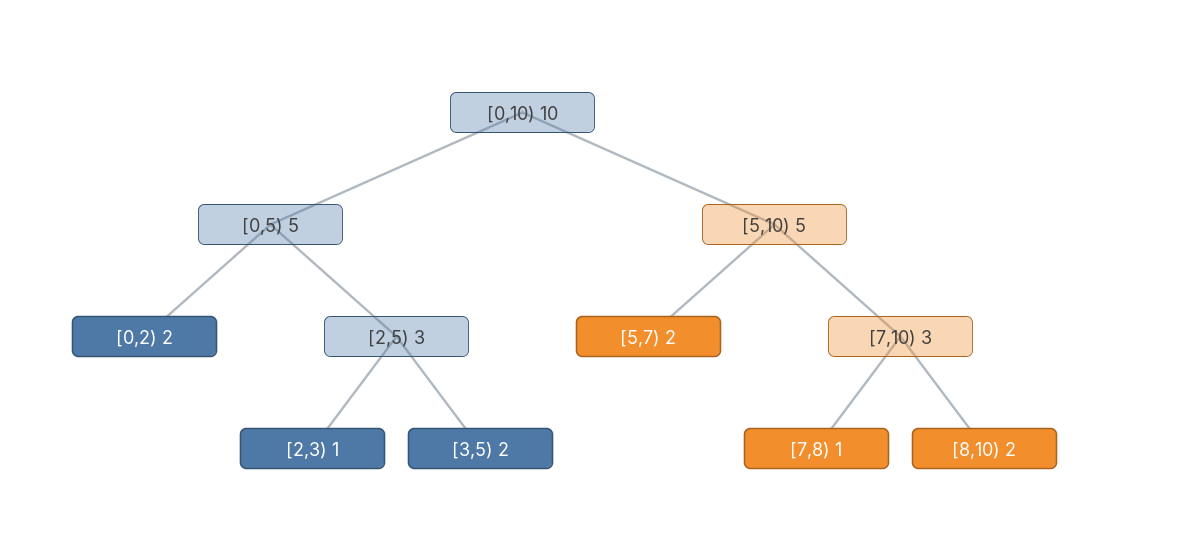
\includegraphics[width=0.78\textwidth]{../docs/images/fig_book_merge.png}
\caption{Жишээ 1 --- Mergesort, номын 10 элементтэй жишээ, threshold $=2$.
Мод бүрэн тэгш хэмтэй. Хоёр өнгө нь хоёр ажилчин урсгалыг заана.}
\end{figure}

\subsection{Жишээ 2 --- ижил өгөгдөл дээр Quicksort}
Зөвхөн \texttt{Алгоритм}-ыг Quicksort болгоод дахин ажиллуулна.

\begin{figure}[h]\centering
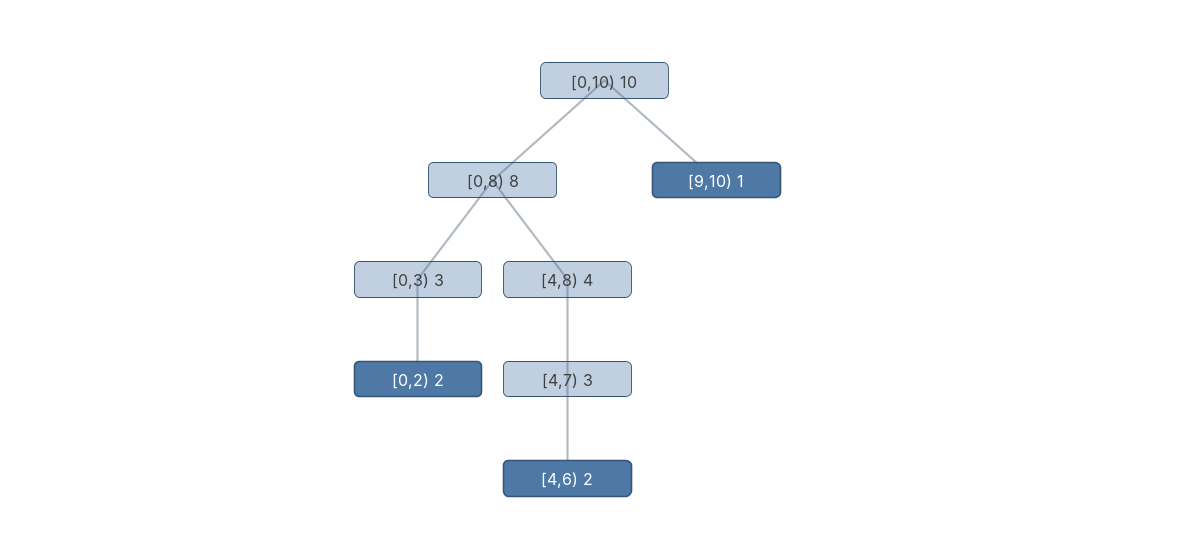
\includegraphics[width=0.70\textwidth]{../docs/images/fig_book_quick.png}
\caption{Жишээ 2 --- Quicksort, ижил өгөгдөл. Мод \emph{тэгш бус}: хуваалт
pivot-оос хамаарна. Зарим зангилаа ганц хүүхэдтэй --- нөгөө тал нь хоосон болсон.}
\end{figure}

\subsection{Жишээ 3 --- threshold-ийн нөлөө}
$n = 400$, Mergesort дээр threshold-ийг $25 \to 5$ болгоход мод \emph{хоёр
түвшин өндөрсөж}, навчны тоо дөрөв дахин нэмэгдэнэ. Энэ бол рекурсийн гүн
threshold-оос хэрхэн хамаарахын шууд нотолгоо.

\subsection{Түгээмэл алдаа ба шийдэл}
\begin{center}
\small
\begin{tabular}{L{5.2cm}L{9.3cm}}
\toprule
Алдаа & Шийдэл \\
\midrule
\texttt{javac: command not found} & JDK суугаагүй эсвэл \texttt{PATH}-д байхгүй.
\texttt{java -version} шалгана. \\
\texttt{UnsupportedClassVersionError} & JDK 17-оос доош хувилбар. Шинэчилнэ. \\
Цонх нээгдэхгүй, \texttt{HeadlessException} & Дэлгэцгүй орчин (SSH).
\texttt{--headless} эсвэл \texttt{--render} горимыг ашиглана. \\
``Threshold хамгийн багадаа 1 байна'' & 0 эсвэл сөрөг утга оруулсан.
0 бол рекурс хэзээ ч зогсохгүй тул зөвшөөрөхгүй. \\
``Бүхэл тоо биш утга'' & Өөрийн оролтод тоо биш тэмдэгт байна. Алдааны
мэдээлэлд хэд дэх байрлалд байгааг заана. \\
Мод хэтэрхий нягт, уншигдахгүй & Дугуйгаар томруулах, эсвэл $n$-ийг
багасгах / threshold-ийг өсгөх. \\
\texttt{StackOverflowError} & Маш жижиг threshold ($=1$) ба маш том $n$ үед.
\texttt{java -Xss16m} гэж стекийг томсгоно (\texttt{run.sh} дотор аль хэдийн бий). \\
Хурдасгалт 1-ээс бага & Threshold хэт жижиг эсвэл $n$ хэт бага --- fork-ийн
зардал давамгайлж байна. Threshold-ийг 50--500 болгоно. \\
\bottomrule
\end{tabular}
\end{center}

\end{document}
